% Chapter 1

\chapter{Introduction} % Chapter title

\label{ch:introduction} % For referencing the chapter elsewhere, use \autoref{ch:introduction}

\section{Introduction}
\subsection{What is machine learning}
\begin{example}
\quad
\begin{itemize}
  \item Database mining: Large datasets from growth of automation / web.
      \begin{itemize}
        \item \Eg Web click data, medical records, biology, engineering.
      \end{itemize}
  \item Applications can't program by hand.
      \begin{itemize}
        \item \Eg Autonomous helicopter, handwriting recognition, most of Natural Language Processing (NLP), Computer Vision.
      \end{itemize}
  \item Self-customizing programs.
        \begin{itemize}
          \item \Eg Amazon, Netflix product recommendations.
        \end{itemize}
  \item Understanding human learning (brain, real AI).
\end{itemize}
\end{example}

\begin{definition}(Informal Definition)

Machine Learning: Field of study that gives computers the ability to learn without being explicitly programmed. (Arthur Samuel, 1959)
\end{definition}

\begin{definition}
\quad
Well-posed Learning Problem is defined as follows.
A computer program is said to learn from experience $E$ with respect to some task $T$ and some performance measure $P$, if its performance on $T$, as measured by $P$, improves with experience $E$. (Tom Mitchell, 1998)
\end{definition}

\subsection{Supervised learning vs unsupervised learning}
\begin{definition} Machine learning algorithms:
\begin{itemize}
  \item Supervised learning: "right answer" is given.
      \begin{itemize}
        \item Regression: Predict continuous valued output.
        \item Classification: Discrete valued output (0 or 1, etc.).
      \end{itemize}
  \item Unsupervised learning: "right answer" is not given - there is no feedback based on the prediction results.
      \begin{itemize}
        \item Clustering: Take a collection of different genes, and find a way to group genes into groups that are similar or related.
        \item Non-clustering: The "Cocktail Party Algorithm", allows you to find structure in a chaotic environment.
      \end{itemize}
  \item Others: Reinforcement learning, recommender systems
\end{itemize}
\end{definition}

\section{Linear regression with one variable}
\subsection{Model representation}
\begin{itemize}
  \item \textbf{Training set}: the data set in supervised learning.
  \item $m$: Number of training examples
  \item $x$: "input" variable/features
  \item $y$: "output" variable/ "target" variable
  \item $(x^{(i)},y^{(i)})$: $i^{th}$ training example
\end{itemize}

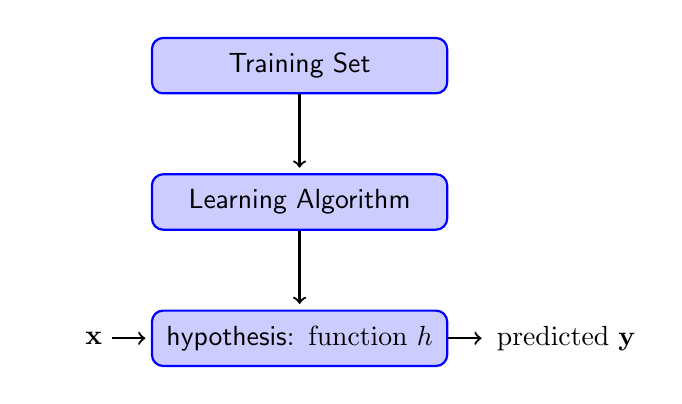
\begin{tikzpicture} [
    auto,
    block/.style    = { rectangle, draw=blue, thick,
                        fill=blue!20, text width=10em, text centered,
                        rounded corners, minimum height=2em },
    line/.style     = { draw, thick, ->, shorten >=2pt },
  ]
  % Define nodes in a matrix
  \matrix [column sep=5mm, row sep=10mm] {
                   & & \node [block] (Training) {\textsf{Training Set}}; & \\
                   & & \node [block] (Learning) {\textsf{Learning Algorithm}}; & \\
            &\node (input) {\textbf{x}};
                    & \node [block] (h) {\textsf{hypothesis}: function $h$};
            & \node (output) {\text{predicted \textbf{y}}};\\
  };
  % connect all nodes defined above
  \begin{scope} [every path/.style=line]
    \path (Training)    --    (Learning);
    \path (Learning)    --    (h);
    \path (input)       --    (h);
    \path (h)           --    (output);
  \end{scope}

\end{tikzpicture}


\textbf{How do we represent $h$?} Linear regression with one variable (Or univariate linear regression)
$$h_{\theta}(x)=\theta_0+\theta_1 x$$



\subsection{Cost function}

\begin{itemize}
  \item Hypothesis: $h_{\theta}(x)=\theta_0+\theta_1 x$
  \item Parameters: $\theta_i$'s
\end{itemize}

Question: How to choose $\theta_i$'s?

Idea: Choose $\theta_0$, $\theta_1$ so that $h_{\theta}(x)$ is close to $y$ for training examples $(x,y)$.
$$\min_{\theta_0, \theta_1} J(\theta_0, \theta_1)$$
where
\begin{itemize}
  \item $J(\theta_0, \theta_1)=\frac{1}{2m}\sum^m_{i=1}(h_\theta(x^{(i)})-y^{(i)})^2$: cost function/ squared error function
  \item $h_{\theta}(x^{(i)})=\theta_0+\theta_1 x^{(i)}$
\end{itemize}

\subsection{Gradient descent}

Question: Have some function $J(\theta_0, \theta_1)$, want $\min_{\theta_0, \theta_1} J(\theta_0, \theta_1)$.

Outline:
\begin{itemize}
  \item Start with some initial $\theta_0, \theta_1$ (a common choice would be setting $\theta_0=0, \theta_1=0$).
  \item Keep changing $\theta_0, \theta_1$ to reduce $J(\theta_0, \theta_1)$ until we hopefully end up at a minimum.
\end{itemize}

\textbf{Gradient descent algorithm}:

Repeat until convergence \{
$$\theta_j\coloneqq\theta_j-\alpha\frac{\partial}{\partial \theta_j}J(\theta_0,\theta_1)\quad (for\ J=0,\  j=1)$$
\}

where $\alpha$ is learning rate.

\textbf{Simultaneous update:}
\begin{enumerate}
  \item $temp0\coloneqq\theta_0-\alpha\frac{\partial}{\partial \theta_0}J(\theta_0,\theta_1)$
  \item $temp0\coloneqq\theta_1-\alpha\frac{\partial}{\partial \theta_1}J(\theta_0,\theta_1)$
  \item $\theta_0\coloneqq temp0$
  \item $\theta_1\coloneqq temp1$
\end{enumerate}

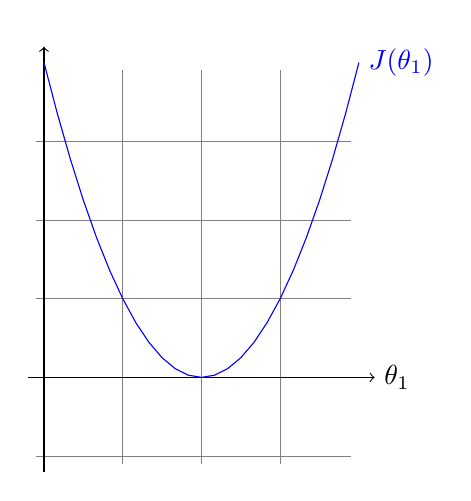
\begin{tikzpicture}[domain=0:4]
  \draw[very thin,color=gray] (-0.1,-1.1) grid (3.9,3.9);
  \draw[->] (-0.2,0) -- (4.2,0) node[right] {$\theta_1$};
  \draw[->] (0,-1.2) -- (0,4.2) node[above] {};
  %\draw[color=red]    plot (\x,\x)             node[right] {$f(x) =x$};
  % \x r ????
  \draw[color=blue]   plot (\x,{(\x-2)^2})    node[right] {$J(\theta_1)$};
  %\draw[color=orange] plot (\x,{0.05*exp(\x)}) node[right] {$f(x) = \frac{1}{20} \mathrm e^x$};
\end{tikzpicture}